\chapter{Aralia Benchmarks -- Revisited}

\section{Accuracy Benchmark}
\begin{landscape}
\begin{figure}[p]
    \centering
    \includegraphics[width=1.38\textwidth]{figs/aralia/rel_log_error_vs_prob.png}
    \caption{Absolute error (Log-probability) for \acrfull{dpmc} vs \acrfull{mcub} and \acrfull{rea}}
    \label{fig:canopy_rel_error_plot_revies}
\end{figure}
\end{landscape}

\section{Convergence Runs}
%% rel_margin_err = 0.001 * \hat{p}
%% CI 0.99
%% timeout 60 seconds
In this section we revisit the Monte--Carlo convergence experiments on the \emph{Aralia} fault--tree data set (Section~\ref{subsec:aralia_dataset}).  The original study targeted a relative margin of error of $0.1\,\%$\,---that is, $\varepsilon = 10^{-3}\,\hat{p}$---at a $99\,\%$ confidence level with a wall--clock time limit of 60~s per model.  Those criteria are maintained here to allow a like--for--like comparison while isolating the impact of the solver refinements introduced in this second iteration.

Figures~\ref{fig:conv_fig_01} and~\ref{fig:conv_fig_02} are the updated convergence traces for \texttt{baobab1} and \texttt{baobab2}, the first two of the Aralia fault trees.  Each plot traces a timestamped run belonging one of the Aralia models.
\begin{itemize}
  \item the sample mean estimate (solid colored line),
  \item the empirical $90\,\%$ and $99\,\%$ confidence bands (shaded regions), and
  \item where available, the reference ``true/known'' probability (black dashed), for comparison.
\end{itemize}

The remainder of the 41 convergence runs can be located in Appendix \ref{chap:revised_aralia_benchmark_plots}.

\begin{landscape}

%% conv_fig_01
\begin{figure}
    \centering
    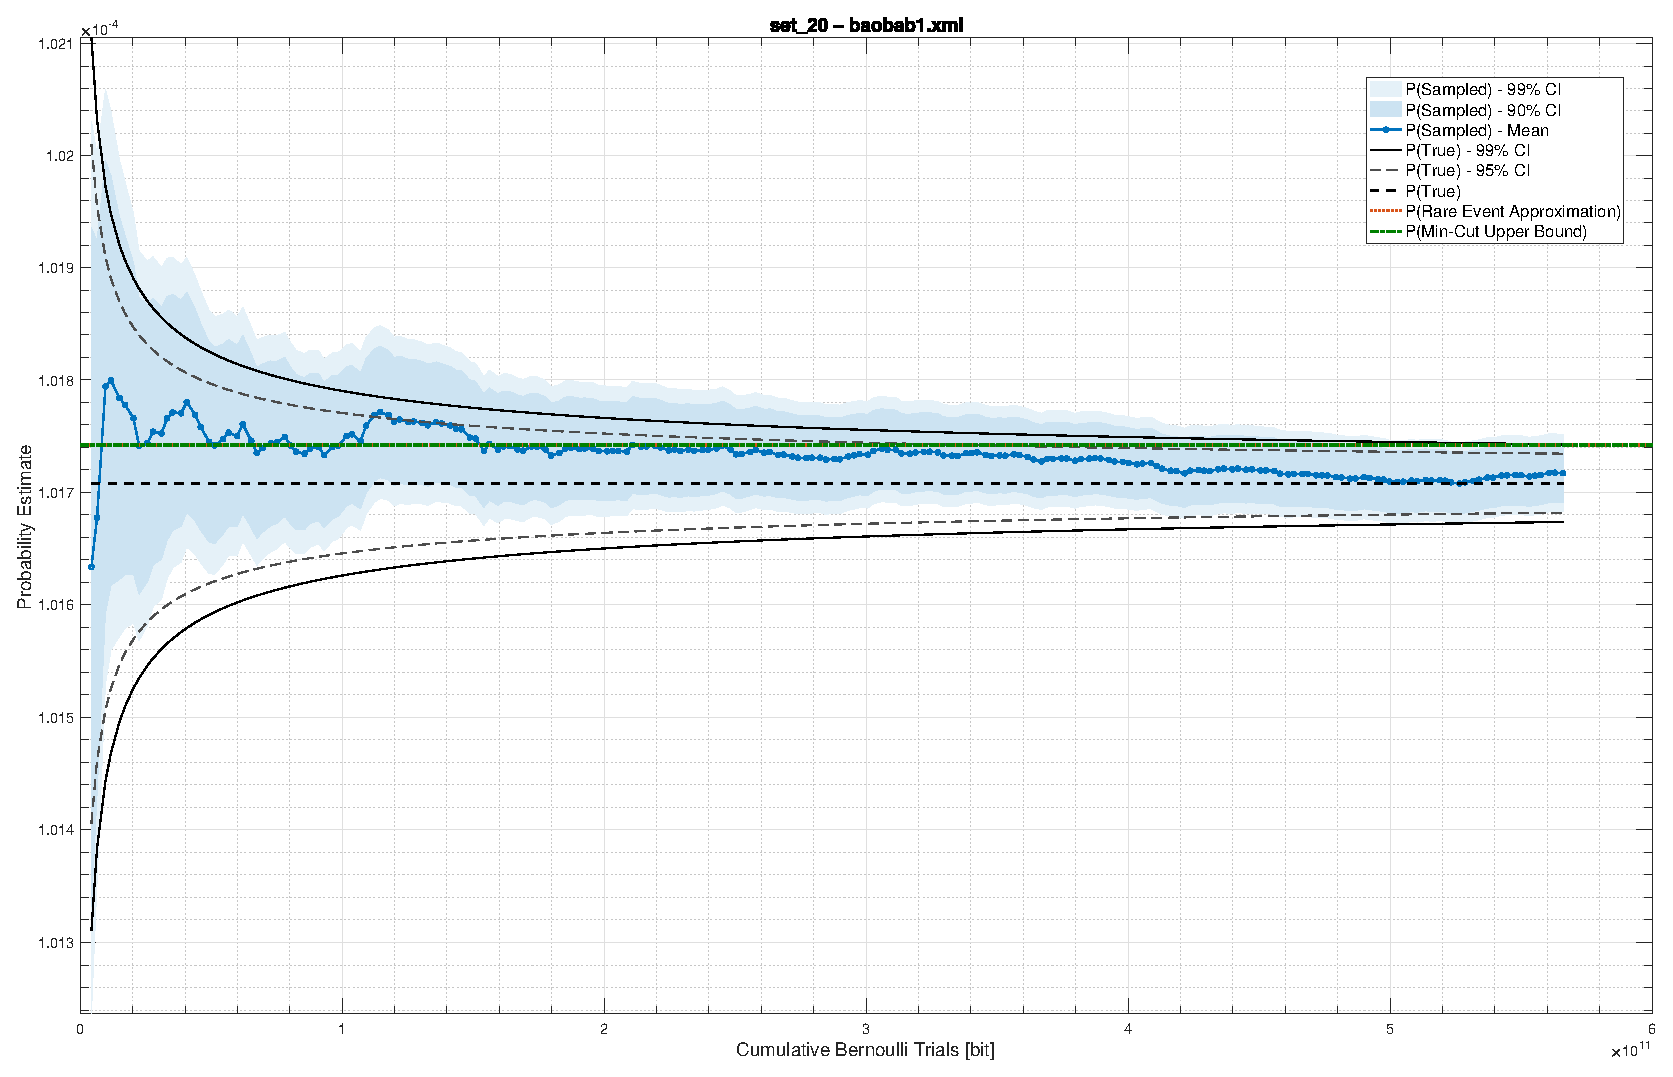
\includegraphics[width=1\textwidth]{figs/convergence/e001p99/conv_fig_01.eps}
    \caption{Convergence trace for \texttt{baobab1}, with 60 second timeout.}
    \label{fig:conv_fig_01}
\end{figure}

%% conv_fig_02
\begin{figure}
    \centering
    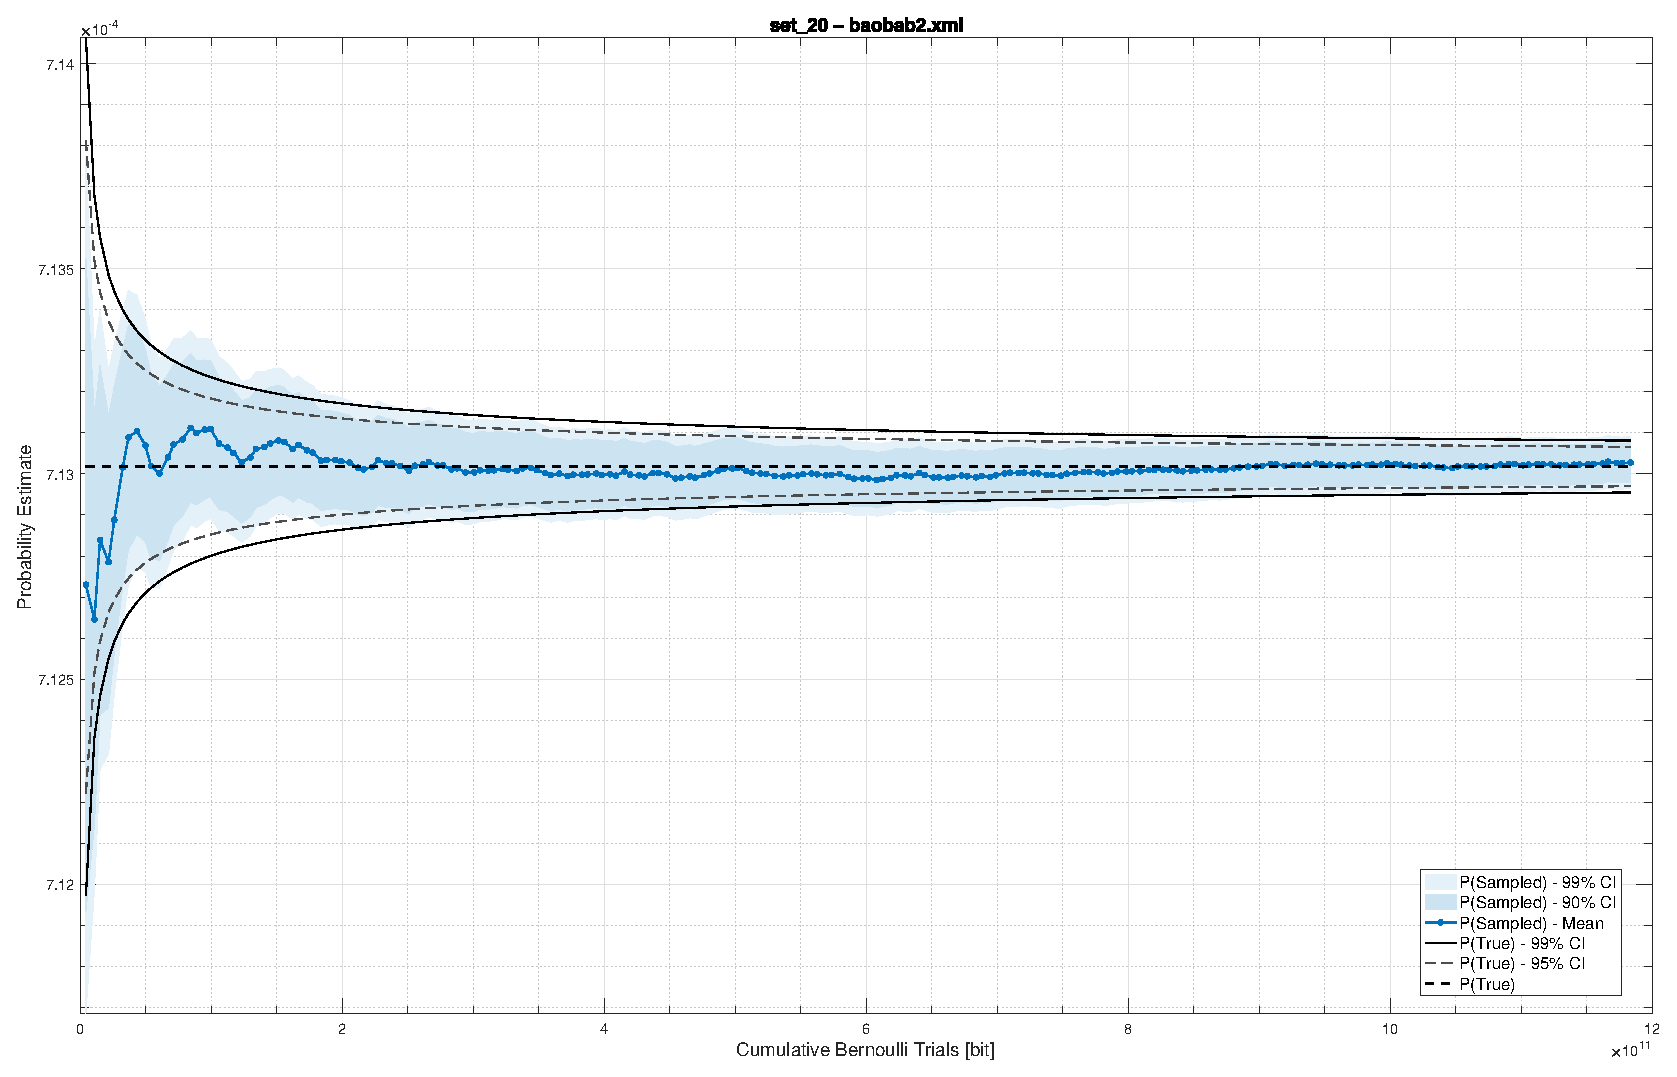
\includegraphics[width=1\textwidth]{figs/convergence/e001p99/conv_fig_02.eps}
    \caption{Convergence trace for \texttt{baobab2}, with 60 second timeout.}
    \label{fig:conv_fig_02}
\end{figure}
\end{landscape}


\section{Throughput Benchmark}
\clearpage
\begin{landscape}
\begin{figure}[p]
    \centering
    \includesvg[width=\linewidth]{figs/aralia/throughput_vs_nodes_by_device.svg}
    \caption{Throughput as function of graph size on multicore CPUs, embedded GPUs, and various discrete GPUs}
    \label{fig:nodes_vs_throughput}
\end{figure}
\end{landscape}

\begin{landscape}
\begin{figure}[p]
    \centering
    \includegraphics[width=\linewidth]{figs/aralia/slides_nodes_vs_convergence.eps}
    \caption{Time to convergence as a function of graph size for varying convergence targets on multicore CPUs, embedded GPUs, and a discrete GPU}
    \label{fig:nodes_vs_convergence}
\end{figure}
\end{landscape}
